% This file was created with tikzplotlib v0.10.1.
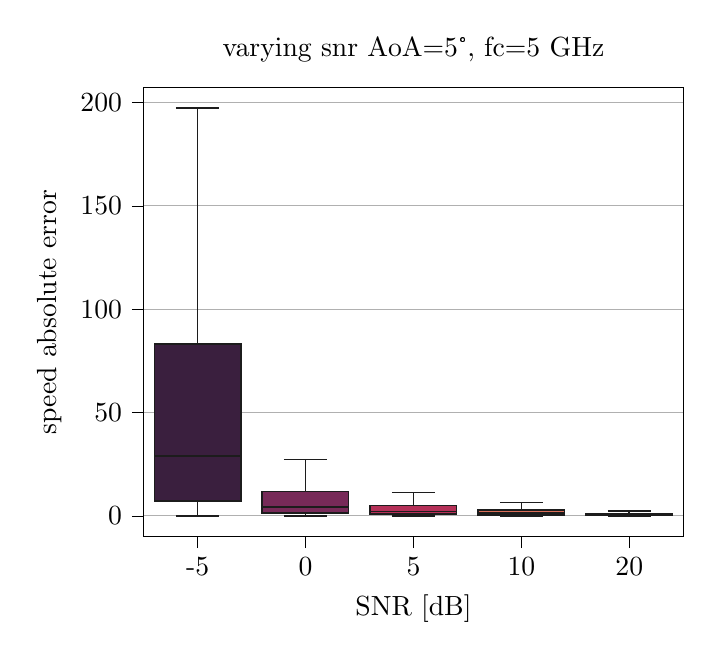
\begin{tikzpicture}

\definecolor{black28}{RGB}{28,28,28}
\definecolor{brown1814888}{RGB}{181,48,88}
\definecolor{burlywood231175145}{RGB}{231,175,145}
\definecolor{darkgray176}{RGB}{176,176,176}
\definecolor{darkslategray583162}{RGB}{58,31,62}
\definecolor{indianred21811088}{RGB}{218,110,88}
\definecolor{purple1194288}{RGB}{119,42,88}

\begin{axis}[
tick align=outside,
tick pos=left,
title={varying snr AoA=5°, fc=5 GHz},
x grid style={darkgray176},
xlabel={SNR [dB]},
xmin=-0.5, xmax=4.5,
xtick style={color=black},
xtick={0,1,2,3,4},
xticklabels={-5,0,5,10,20},
y grid style={darkgray176},
ylabel={speed absolute error},
ymajorgrids,
ymin=-9.86042000132069, ymax=207.068917757608,
ytick style={color=black}
]
\path [draw=black28, fill=darkslategray583162, semithick]
(axis cs:-0.4,7.26457276645877)
--(axis cs:0.4,7.26457276645877)
--(axis cs:0.4,83.242460076005)
--(axis cs:-0.4,83.242460076005)
--(axis cs:-0.4,7.26457276645877)
--cycle;
\path [draw=black28, fill=purple1194288, semithick]
(axis cs:0.6,1.46563379901044)
--(axis cs:1.4,1.46563379901044)
--(axis cs:1.4,11.8161565841415)
--(axis cs:0.6,11.8161565841415)
--(axis cs:0.6,1.46563379901044)
--cycle;
\path [draw=black28, fill=brown1814888, semithick]
(axis cs:1.6,0.785049937222727)
--(axis cs:2.4,0.785049937222727)
--(axis cs:2.4,4.99031808520913)
--(axis cs:1.6,4.99031808520913)
--(axis cs:1.6,0.785049937222727)
--cycle;
\path [draw=black28, fill=indianred21811088, semithick]
(axis cs:2.6,0.457113761706436)
--(axis cs:3.4,0.457113761706436)
--(axis cs:3.4,2.86958731614837)
--(axis cs:2.6,2.86958731614837)
--(axis cs:2.6,0.457113761706436)
--cycle;
\path [draw=black28, fill=burlywood231175145, semithick]
(axis cs:3.6,0.154669638287864)
--(axis cs:4.4,0.154669638287864)
--(axis cs:4.4,0.975065494430688)
--(axis cs:3.6,0.975065494430688)
--(axis cs:3.6,0.154669638287864)
--cycle;
\addplot [semithick, black28]
table {%
0 7.26457276645877
0 0.000642015990285572
};
\addplot [semithick, black28]
table {%
0 83.242460076005
0 197.20849331402
};
\addplot [semithick, black28]
table {%
-0.2 0.000642015990285572
0.2 0.000642015990285572
};
\addplot [semithick, black28]
table {%
-0.2 197.20849331402
0.2 197.20849331402
};
\addplot [semithick, black28]
table {%
1 1.46563379901044
1 5.73306725657474e-05
};
\addplot [semithick, black28]
table {%
1 11.8161565841415
1 27.3137452638486
};
\addplot [semithick, black28]
table {%
0.8 5.73306725657474e-05
1.2 5.73306725657474e-05
};
\addplot [semithick, black28]
table {%
0.8 27.3137452638486
1.2 27.3137452638486
};
\addplot [semithick, black28]
table {%
2 0.785049937222727
2 0.000158163369309072
};
\addplot [semithick, black28]
table {%
2 4.99031808520913
2 11.2921075556963
};
\addplot [semithick, black28]
table {%
1.8 0.000158163369309072
2.2 0.000158163369309072
};
\addplot [semithick, black28]
table {%
1.8 11.2921075556963
2.2 11.2921075556963
};
\addplot [semithick, black28]
table {%
3 0.457113761706436
3 4.44226696849626e-06
};
\addplot [semithick, black28]
table {%
3 2.86958731614837
3 6.47375702082791
};
\addplot [semithick, black28]
table {%
2.8 4.44226696849626e-06
3.2 4.44226696849626e-06
};
\addplot [semithick, black28]
table {%
2.8 6.47375702082791
3.2 6.47375702082791
};
\addplot [semithick, black28]
table {%
4 0.154669638287864
4 4.31804922467194e-05
};
\addplot [semithick, black28]
table {%
4 0.975065494430688
4 2.20500071359116
};
\addplot [semithick, black28]
table {%
3.8 4.31804922467194e-05
4.2 4.31804922467194e-05
};
\addplot [semithick, black28]
table {%
3.8 2.20500071359116
4.2 2.20500071359116
};
\addplot [semithick, black28]
table {%
-0.4 28.8358002310713
0.4 28.8358002310713
};
\addplot [semithick, black28]
table {%
0.6 4.23617316585331
1.4 4.23617316585331
};
\addplot [semithick, black28]
table {%
1.6 2.16263154271026
2.4 2.16263154271026
};
\addplot [semithick, black28]
table {%
2.6 1.25992823895566
3.4 1.25992823895566
};
\addplot [semithick, black28]
table {%
3.6 0.431940376260191
4.4 0.431940376260191
};
\end{axis}

\end{tikzpicture}
